\section{Chapter 4: What is Trash
Magic?}\label{chapter-4-what-is-trash-magic}

\subsection{Why Trash?}\label{why-trash}

Who owns a dog turd left on the street? Who owns the piles of plastic
bottles that collect in an eddy of an urban stream? Who owns the soot
that collects on the walls of a bus stop? No one. The concept of private
property, which I regard as evil, does not incorporate all things. For
capitalism to function it has to have both ``assets'' and
``liabilities'', which the capitalists associate with opposite signs of
numbers. What if a turd is not a liability or an asset? It does not
exist in the capitalist universe, it is their ultimate trash, of value
to no one, and it is the seed that we must use to create a better world.

\subsection{Why Magic?}\label{why-magic}

Many reasons. First of all, what exactly is magic? It's subjective.
Magic is what, subjectively, gives us a certain feeling of wonder about
the world. I believe that that wonder should be intrinsic to our
technology always, just as we expect it to be with art. Hence the
removal of the artificial separation between art and technology is a
path to what is essentially a form of magic.

Also, the use of this word is very annoying to members of the
technocratic priesthood which this work seeks to undermine. The very
possibility that someone might do something useful and interesting in a
sphere called magical is upsetting to them, because it is clearly not
part of their ``pure'', ``rational'' world. This thus draws a line in
the sand of sorts: on one side is engineering and business and the rest
of the ``rational world'', and our work stands very much on the other
side, where things are a little less sharp and clear and countable.
Hence my statements in the first chapter about Trash Magic being an
artistic movement in this first stage.

\subsection{What is a Trash Witch? What is a Trash
Wizard?}\label{what-is-a-trash-witch-what-is-a-trash-wizard}

Witches and Wizards have for centuries been symbols of humans' ability
to wield various magic powers. I draw on many traditions for this
concept, from pagan lore through Tolkien and Harry Potter. The
traditions built up from fiction, culture, and religions of various
kinds give us a picture to draw on for the archetype of the Trash
Magician. I don't want to use the term ``magician'' too much though
because it can be mistaken for the person who puts on a magic show.
Perhaps that is not all bad, though! The magic show can both teach and
inspire wonder and that is certainly one goal of Trash Magic.

A potential downside of calling us all witches and wizards is that those
can be gendered terms, and that's not what I'm looking for with this new
society. But I will propose for the sake of this work a non gendered
definition of witch and wizard. The person wielding trash magic at any
time is practicing witchery or wizardry if they are doing witch like
magic or wizard like magic.

What?

Well, for example, let's say you're in the woods at night, doing some
hard core potion making and saying something like ``fair is foul and
foul is fair'', and there's a lot of cackling. That's witchery. If
you're in a huge field of rocks swinging your Trash Staff around and
launching lighting bolts at the other rocks, that's wizardry. It doesn't
matter what gender the practitioner may or may not have--if you are
wizarding you're a wizard, if you're witching you're a witch. At least
for the moment. Mostly trash magicians have both Trash Wizard and Trash
Witch natures, and most magics we practice will use both as well.

But I have still only loosely defined this way of being. The Trash witch
is someone who believes in a world where we both have a element of
adventure and mystery in our lives and where we have the advantages of
what we now call ``modern technology''. We believe that this magic
should be available freely to everyone in the world, and that everyone
in the world should have the freedom to wield this and modify it as they
see fit, and use or not use whatever magic they need or don't need.

Trash Wizards and Trash Witches use the laws of physics and the methods
of applied physics as a form of magic. We teach that magic to others,
and spread both the serious scholarship of Trash Magic and the basic
practical skills needed to give the magic to all.

All our teaching and building is free. Free, meaning outside the money
system and capitalist economy. But also free meaning people have total
freedom to take this and duplicate it and modify it and make it truly
their own. A love of pure science demos is a core value of the Trash
Wizard or Witch.

Another goal is independence. A group of just Trash Witches should for
example be able to live on their own, with a good quality of life. Maybe
dozens of Wizards or dozens of Witches can easily form tribes to build
and scavenge and do adventures and art. But also tribes can form
super-tribes which merge to build truly large works. The only way giant
social structures can be optional and not control us all is for us to be
able to live freely with just a few people. The magic we plan to wield
here is designed to give people that power.

\begin{figure}[htbp]
\centering

\includegraphics{images/wizardcartoon.png}
\caption{Wizard by the creek}
\end{figure}

We also strive to amuse. You don't want to learn about magnetic fields
just for the hell of it or just because they're useful. You can see from
us that they're actually magical! Magical enough that a show put on with
magnetic fields or electric fields is very much worth watching. In fact,
one of the most popular shows in most science museums is the electric
field demonstrations with giant lighting machines.

So a Trash Magician uses a combination of Wizardry and Witchery to amuse
and provide for people with Trash of the world. Trash is generally stuff
that is not only free but infinitely free. Not only can you go find one
or two or 10,000 of a thing, you know that later you can go back and do
that again as many times as you want. This is true with flowing water
from spring snow runoff or from tides or drainage of some large rainy
area. It's true of winds that always blow, of the sun, of sand and dirt
and rocks. It's true of sticks shed by the lower sections of pine trees.
And it's true of the plastic bottles thrown away by capitalist society.

A society of free stuff is not one with ``zero cost''. It's one where
cost is infinite but value is also infinite. We are moving to a value
system that works mostly with infinities. That is part of what makes
Trash Magic actually magical. And if you're a Trash Witch or Wizard,
that's your stuff! You wield the magic that moves the trash around!

In addition to Trash Wizardry and Witchery one might be a Trash Daemon
or Trash Imp. Trash Goblins can have a place in our community but not
Trolls.

Trash Wizards are always there for everyone. We welcome the refugees of
capitalism and it's evil twin, war. We do not recognize the validity of
borders and are here to help subvert them as needed to help the down
trodden.

\subsection{Alchemy, Chemistry and Art}\label{alchemy-chemistry-and-art}

Part of the narrative we learn when we study chemistry in school is that
of the failure of alchemy to accurately describe the elements. We learn
that these primitive pre-chemists thought of the elements as being
earth, air, fire and water, rather than the array of chemical elements
we know in today's periodic table. The \emph{real} elements are divided
up based on our supposedly superior modern understanding that atoms are
the basis of all matter.

I dispute none of basic science we all learned in school in terms of
atomic structure, this manifesto is not quite that kooky. What I do
dispute is how information is organized in our minds and in our equation
system. Consider an element like oxygen. We know that a lot of oxygen in
the world around us is in the form of two atoms together, as a gas which
makes up about one fifth of the air around us. We also know that all
water has one oxygen atom(along with two hydrogens), and so all the
water in our world has oxygen. Fire is pretty much always a rapid
chemical reaction involving oxygen, so we also know that all the flames
we see in our world on Earth are partly made from a form of oxygen.
Finally, the one of the most common minerals on our planet is the
relatively inert silicon dioxide that makes up most sand as well as many
other minerals. The melting point of this solid is well over one
thousand degrees.

Now, while I would never deny that it's useful to say all these things
have oxygen, or to understand what that means, is that really the most
pertinent quality they all have? To the alchemist sand is ``earth'',
fire is fire, water is water, and air is air. Four elements, which we
deal with very differently in all possible ways. We look at that and say
it's ``wrong'' because the knowledge of what atoms make up these things
is somehow more ``fundamental'' supposedly. But what if we didn't
organize things that way, even though we understand how atoms work? What
if we still recognized that earth, air, water, and fire as elements,
which just happen to be also made up of atoms? This world view would
have the same facts as the one we hold today, just with their order
re-arranged.

Ideally what I seek from this project is to remove these kinds of
hierarchies altogether. I don't want to say that alchemy is ``right''
and chemistry is ``wrong'', what I object to is the basic notion of
right and wrong here. It's based on the notion of our ideas having some
kind of objective other reality beyond that of the world we live in. I
think this kind of ordering of ideas is one of the ways we've held
ourselves back in science due to ideology.

We need to stop banishing things like spells and elementals and potions
from ``real'' science just because of cultural values. A drug is a magic
potion, what else would it be? Prove it isn't! A program on the firmware
of a robot is a magic spell. Prove it isn't! And every artist knows art
is magic. The only way we have denied that in science is by simply
saying we're better than art on the ladder of ``reality''. This has,
again, held us all back. It's led to a century of inaccessible art and
incomprehensible science. We need to reunite the strands of alchemy,
magic, art, and science.

\subsection{Symbology}\label{symbology}

Where to trash magic artists get our symbols? From the natural world,
from geometry, from anarchist iconography, and from religious art. We
also seek to replicate, but softened by the influence of the natural
world, the design aesthetics of 20th century industry. This will be
almost a parody or a three dimensional rhyme of sorts, not so much to
bring out the function of the industrial thing but to remind us of its
form to make us think of where our trash comes from and what we are
replacing.

Note that when I say religious art, this is very broad, since much of
art through the ages has always been inspired by whatever the artist
viewed religion to mean. Religion is our deepest held beliefs which form
our world view outside of that which can be proven. Art at its best
tries to express what that means, and is often deeply religious, but
takes very different forms due to the diversity of religious beliefs. In
particular, however, trash magic will lean toward the ``occult'' from
various Western traditions. Due to the author's non-indigenous Western
background, I want to avoid appropriating cultural traditions of which
I'm not a part. And I feel like one way to do this is to focus on
``pagan'' traditions of various kinds, as well as occult Jewish and
Christian art.

The anarchist symbology will include the black wild cat used by the IWW
and other anarchists, as well as various permutations of the circle A.
The following image combines the black cat with the form of the magnetic
field from a tiny magnet, symbolizing one of the forces which we will
harness in Trash Magic.

\begin{figure}[htbp]
\centering
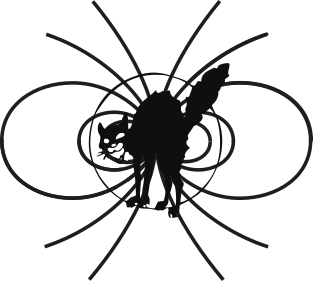
\includegraphics{images/cat3.png}
\caption{Wildcat in the field}
\end{figure}

\begin{figure}[htbp]
\centering

\includegraphics{images/elements.png}
\caption{Elements}
\end{figure}

\begin{figure}[htbp]
\centering

\includegraphics{images/squat.png}
\caption{Squat Sign}
\end{figure}

Some electrical symbols will also be incorporated, partly since many
things we will make involve building electrical circuits, and building
those symbols into the art makes things self-documenting. While these
form a useful function in helping to make a thing free by documenting
how it's put together, they should never abandon form for function:
circuit documentation should be a work of art as much as a document.

Secret symbolism in occult art at UAA library: BF1623.S9 G45 1987

Art and the occult, UAA library: N8222.M3.S38 1975

\subsection{Capitalisms Unwanted: a Human
Treasure}\label{capitalisms-unwanted-a-human-treasure}

What is a Trash Wizard?

What do we do?

What is best in life, redux

How the trash wizards teach the world our methods

What kind of world we build

Many wizardries, many paths

How does the value circle work?

how do trash wizards spread the value circles?

Specific examples of value circle use: manufacturing, food, robots,
coffee, R\&D, art

Many technical details on trash wizard sticks, how they're used,
designs, plans, images, examples, etc etc. on the sticks.

Use of sticks with cars, computers, phones

using the stick to replace the smart phone eventually

\subsection{What Does the Trash Wizard Stick do and
have?}\label{what-does-the-trash-wizard-stick-do-and-have}

\begin{enumerate}
\def\labelenumi{\arabic{enumi}.}
\item
  built in measuring stick in SI and English
\item
  build in measure tool for AWG of wires
\item
  LRC meter that reads out on phone
\item
  conversion to robot mode where it drives itself around
\item
  convenient single shoulder strap for comfortable wear like a bike
  messenger pack
\item
  random flash sticks which store MP3's of music ripped from youtube on
  the pi, controlled by the smart phone, and then replayed later
\item
  speaker built from our technology, reading flash drives out with the
  pi zero
\item
  pi zero
\item
  High voltage storage caps(detachable)
\item
  medium voltage storage caps(detachable)
\item
  super cap(detacheable)
\item
  LiPo Battery(detacheable)
\item
  direct wire connect silicone and copper switch board for power with
  fail safes of various kinds
\item
  screen for pi zero to read out a special dumb ass bat phone
\item
  measure nonlinear voltage response to impulse of various random blobs
  you find around
\item
  can harvest energy using a built in magnet and coil setup
\item
  water pump always available
\item
  trash wizard app for phone is set up for physics, interfaces with
  existing physics packages
\item
  audio high gain amp with speaker that can get high power sound to do
  feedback
\item
  goggles that can interface with various imaging technology using
  analog displays with vibrating fluids
\item
  L R and C are all measured analog using the high gain audio stick
\item
  measure NOISE of all things, including Johnson and shot noise
\item
\end{enumerate}

\subsection{Trash wizard multi tool}\label{trash-wizard-multi-tool}

I want the trash wizard multi tool to be able to measure inductance
easily. How to do that? I want the L/R time of something to be long
enough to see something on the arduino ADC. But what R? If L is 0.001 H
and R is 1 ohm, L/R is 1 ms. Perhaps a 1 ohm shunt resistor somewhere.

Or maybe I want to measure the reverse EMF from changing the current
quickly through the coil. V = L dI/dT. For a 1k series resistor driven
by 3 V we have 3 mA of current. If that can turn off or on in a few
microseconds, it should be possible to induce a good fraction of a volt.
But given that the sign will reverse, having this go to ground would be
a problem for the ADCs on the arduino. So what I want is a 500 ohm
resistor going from the DAC to a node between two 500 ohm resistors in
series making a voltage divider between 0 V and 3.3 V. that middle node
then goes to the ADC and pulses should be visible. This I will not
proceed to build and test.

\subsection{Free Phones of the Future}\label{free-phones-of-the-future}

One of the many idiotic things capitalists say to shut up their critics
is to point out that capitalism is the source of the smart phones that
anti capitalists inevitably use. These devices are indeed amazing, and
are no longer luxury items by any means. On the contrary, they are very
much a survival tool used by the oppressed classes now, and it's very
dangerous to ignore that role this technology plays. But what aspect of
them is so great? The social networking. That's always what you need:
access to the web, various messaging systems, and various commercial
things like Uber and Lyft.

Does that really need to be a computer? A truly free phone would be a
pure communication tool that communicates in a distributed way like fido
net of old. the sole purpose of the hardware would be to communicate
images, sounds, text, and to decide where those should go. That's it.
What the hell do you need a computer for? Mostly so that The Man can spy
on you and figure out how to sell you shit you don't need, and force you
to constantly throw more federal reserve debt back into the machine for
more advanced machines to get more indoctrination to continue the cycle.

It's all bullshit! Don't be fooled by the dominance of the computer
technology into believing that's inevitable. It's not. We can get orders
of magnitude more benefit from peer to peer networks than we do today as
slaves to the military industrial machine if these phones were all free
like freedom, linked up on free hardware all the way. This can actually
be the basic informational skeleton of the value circles.

I believe that the hardware can be re worked from the ground up based on
our approach to applied electromagnetism to get something with totally
new fab. But in the mean time, given that that is a lengthy applied
physics research project, what can we do? My answer is to watch closely
everything that has anything to do with Raspberry Pi and other
``internet of things'' projects in the open hardware domain. I say
``open hardware'' here and not free hardware, because it's not free
according to my strict definition: it relies on mine- driven fab and
capitalism, and there is IP in the supply chain(and some other
problems). But it's way better in terms of open and free than the whole
android/apple ecosystem.

as seen here: https://www.adafruit.com/products/2885
(https://www.adafruit.com/products/2885) The pi zero sells for 5
dollars! And it's free like freedom as far as the software goes, as I
understand it. The problem of course is that it's not what you'd call a
product still. You need to buy a screen separately, and a battery, and
some other odds and ends, and then put a package together, get all the
software working, etc. It's not trivial. Not insanely hard, but not
trivial and also not really as usable as a apple or android. But surely
this could change? If people want to work within the system of existing
``tech'' a fantastic place to focus efforts would be making this
technology closer to truly free. This will be a combination of figuring
out sourcing logistics on the hardware, making the software closer to
what a phone user expects, and writing new software to make more free
infrastructure that runs on the free hardware. If a truly free platform
were to allow for the kind of peer to peer labor and goods sharing that
for profit platforms now have, capitalism might just collapse overnight
as people spontaneously are able to work and do things by communicating
freely.

Don't like the phone but like ``tech''? make a free phone. It will
happen one way or the other, but the more ways it happens the better for
everyone.

\subsection{How to Build the Team to build the
Technology}\label{how-to-build-the-team-to-build-the-technology}

I'm clearly not going to build all the things I'm describing here. And
even the things I do build, I hope to have what I build be a
insignificant fraction of the total number of units produced in the
future. How to recruit? Who to recruit? Where will they work? I've been
contemplating these questions, and I see several ways to proceed.

Largely the various ways forward will involve decisions about where to
be on the spectrum of working inside the system vs.~outside. Some
choices will involve getting very conventional, and I fear they will end
up being coopted by the existing system. One of those would be to
structure the way ARPA was in ins heyday. Many top academic, corporate,
and government research labs could receive targeted funds to work on
problems, where the funds come from various donations and military
applied science grant money. The work would then be done by the usual
suspects: grad students, post docs, and various staff researchers inside
the current system. I think the biggest danger here is that the
developed technologies will not be free in the real sense because it's
so hard for a expensive R\&D lab to ever build a thing that's not based
on expensive equipment.

Another way forward is to focus on commercial applications in the old
economy. One could for instance build a very reliable and cheap water
pump, and build a rapidly growing for-profit company on that which funds
R\&D to free technology through its profits. This is, I think, the worst
of all possible choices. Capitalism poisons everything it touches. And I
think the way I'm going to define capitalism for the purpose of this
work is ``the belief that value can be measured using numbers''. It's
that simple. Any kind of money or equivalent value unit that can be
counted is the poison we all know from our capitalist nightmare, and
that's what I'm going to focus on purging from the technological supply
chain.

At the other end of the spectrum, one imagines seizing a abandoned
factory building and building the R\&D infrastructure up from scratch in
a squat environment. I predict that going too far down this path ends
with the usual endless war with cops and landlords that always happens
when good people try to use land without the System. Even if you imagine
buying the land so that there are no direct legal challenges, cops and
landlords will be an ever-present problem, as will generating enough
federal reserve debt to keep the bastards off our backs. A lot of time
will have to be spent on just keeping the site running.

Seizing land and building up the means of production makes sense when
you have a working technology that can be instantly deployed and then
also broken down and moved later when you need to move. But before the
technology is mature, it makes sense to be completely distributed
geographically. Also, for this project to work as I want it too, we need
strong cooperation between the developing world and the developed world,
and between diverse people living on land that has different types of
local resources available from whatever their local trash streams are,
as well as the very diverse energy considerations, and the diverse
cultural considerations which should be considered early not later.

How does this distributed system work? I believe part of it involves the
structure of the actual book document. I don't feel that the Jupiter
notebooks are quite where I want them yet, but they're close, and I
think that the structure will be based on software that comes out of
that basic structure. Users will make modules to solve various technical
problems, as well as post new ones, and they'll all be integrated into
the combined book. This is, in many ways, what the open source software
people do using their git hub bullshit. I think git up is a giant
festering piece of shit, however, and loathe most software communities,
so this is a tricky game. Somehow the innovations from that world should
be used without poisoning the whole project and creating yet another
tech bro shit head club.

One way I want to differentiate from a lot of computer software bullshit
is by having a coherent narrative. Something that drives me crazy about
their culture is that things are so distributed that you can't actually
figure out where to start. It's not just that there are forks, it's that
there are many forks all the time for everything and everyone is a giant
dick about all of it. I'm not above simply banning anyone with any tech
company affiliations from contributing to the main document.

This is a book. A book is a finite thing. As time goes on content will
be added, but other content will also be deleted. It will all be
archived, but if someone wants to they can approach from zero, start at
the beginning, and have a coherent narrative to follow as they build up
to actually having the ability to use the technology themselves. There
will be various versions to account for many human languages as well as
some various tracks that might exist, but all of the parallel versions
and tracks must be self contained and linear(or at least with the option
of treating them as linear). I need to keep a very close eye on how
things progress with the various jupiter like things out there, because
it's moving fast. It all has to work on a free trash wizard stick, but
that should be fine with the HTML5 stuff that everything now runs on
inside a browser. Is there a simple way to go back and forth between
jupiter notebooks and a fully compiled .pdf in book format? Surely there
is, and if not, it should be some combination of existing scripts
chained together.

My job as initial author is to create well posed problems in the first
draft of the book, and to make it appealing for people to contribute
solutions to those problems. This will be extremely hard to get right on
a first pass, and part of getting this whole thing to work will involve
shifting that format over time. When things are really working, the R\&D
will be all done in the value circle economy, where people are
constantly creating that form of value as they do R\&D. This has the
potential to be a very hard chicken-and-egg problem: the book needs a
lot of work in order to have value circles work, but without value
circles people can't work on it effectively. That's why this all starts
with me working alone in my underwear at home. And remains that way for
a while. Because I need to first have the system working with me as the
only user, then me and some close associates, then a few ``followers''
who just build kits, and then, when that team has worked for a few
years, more people can ease their way into the system to grow it. Of
course as the serial/parallel global crises of capitalist disaster
accelerate, we may find that things grow explosively instead. If that
happens it happens, but I will plan for something that is built much
more carefully.

This blog post was going to go into a list if the types of experts
needed to get the various jobs done, but on looking where it ended up
going that looks more and more like a useless exercise at this time.
I'll build up the vision of what should get built, build my own parts of
that technology and distribute them, and then a sort of chemical
potential will form which brings in the right experts. It's dangerous to
specify exact professional qualifications too early, as it will end up
losing out on some opportunities to bring in talent outside the
organized technical professions, which creates lots of biases in class,
race, nationality, age, etc. It's much better to pose problems clearly
with no jargon, in as many ways as possible and just see who turns up
with a solution.

\subsection{Skeletron: The Wooden Bones of
Art}\label{skeletron-the-wooden-bones-of-art}

Skeletron is the system that makes the bones of Trash Magic artifacts.
Skeletron is simply a way to modify things found in your environment to
make them play together well with Trash Magic. Primarily this means
gathering sticks, shaving them to be flat on one or more sides and
removing the bark, and drilling holes in them. Quarter inch holes spaced
about one inch along the line of the sticks is the most basic component
of Skeletron. This can be used to do many things, and as more people
build it and use it and modify it, it will become increasingly versatile
and free.

With a universal wood framing system we can build up many different
human sized structures. This can be used to make various shelters,
although to do this we will add plastics to the system, using methods of
hand plastic welding detailed in the last chapter of this volume. With
the ability to make wood skeletons with plastic skins we can make
waterproof structures on land as well as waterproof boat structures and
amphibious artifacts of various kinds. The combination of wood and
plastic in a modular and modifiable way also can be the basis of all the
other industrial constructions to be described in this work.

The fasteners to hold the sticks together are all quarter twenty, or one
quarter inch outer diameter threads with 20 threads per inch, a very
common standard in the US. In Metric countries, the equivalent would be
about M6. The M6 and the quarter inch threads are not compatible, but
the hole sizes should be, especially if you drill them out big enough to
have some extra space around the bolts. Bolts and nuts can be stainless
steel if you want to buy some, or melted plastic can be used to make
plastic bolts and nuts and wrenches from bottle caps or other similar
plastics.

In addition to making large sticks with many holes in them and welded
plastic sheets for water tight construction, we have a system for
building electronics directly into the sticks. This involves some
soldering techniques detailed in the last chapter of this volume as
well, as well as the plastic welding techniques to fix in place, strain
relieve and protect the circuits as needed.

A drill is needed for this work to cut the quarter inch holes for the
main Skeletron sticks as well as to make smaller holes for various wires
and components for the electrical circuits. While it can be easy with
Grid access to use a simple electric power drill, the ideal Trash Magic
industrial production will involve a direct drive drill driven by
flowing water.
